\documentclass[Main]{subfiles}
\begin{document}

\subsection{SekvensDiagrammer}

\subsubsection{Use case 1 -- Init drone}

\begin{figure}[H]
\centering
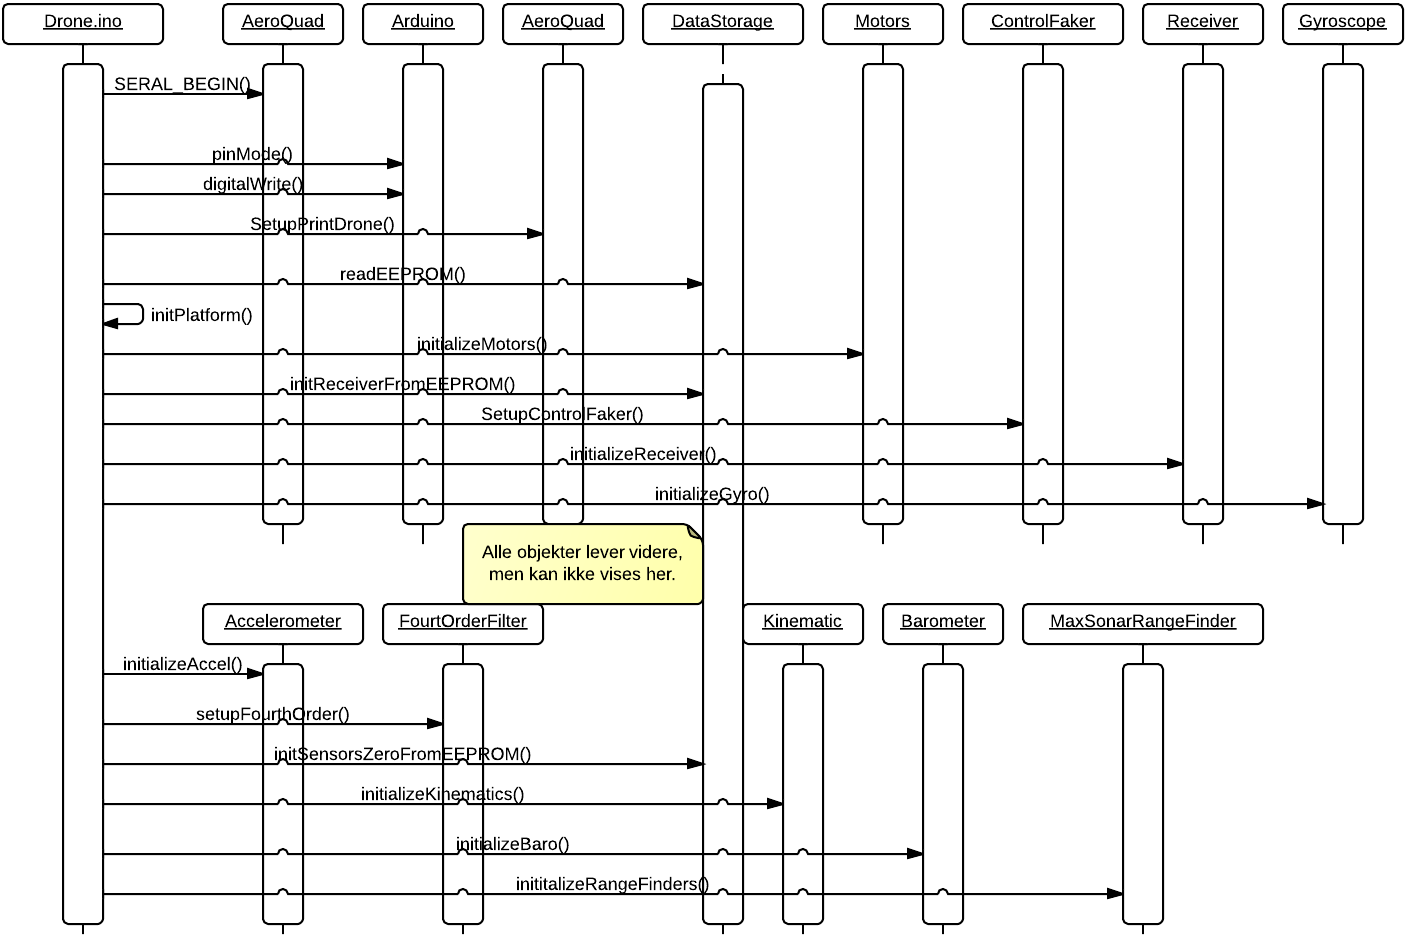
\includegraphics[angle=90, scale = 0.55]{SekvensInit}
\caption{Init af drone}
\label{Fig:SekvInit}
\end{figure}

På Figur \ref{Fig:SekvInit} ses de kald der foretages, når dronen starter op første gang den får strøm.
Efter initieringen startes Arduino's \code{loop()}-funktion, der kører i ring til strømmen afbrydes, som vist på Figur \ref{Fig:SekvDroneHz}.


\begin{figure}[htbp]
\centering
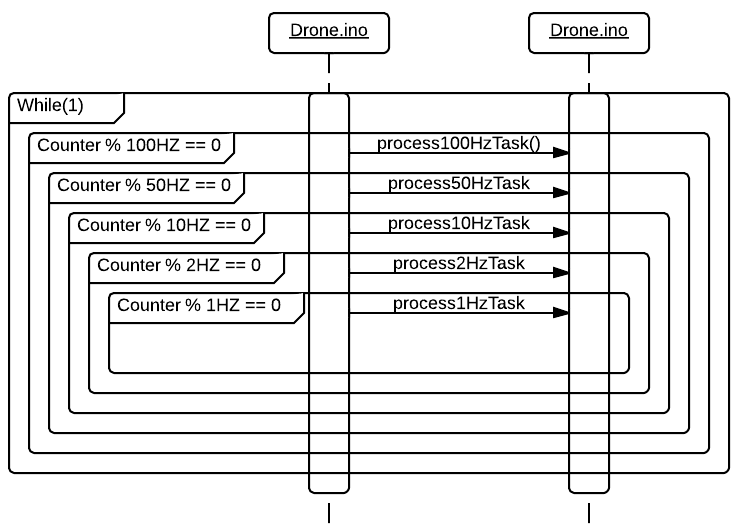
\includegraphics[scale = 0.55]{DroneLoop}
\caption{Schedulering i \code{loop()}-funktionen}
\label{Fig:SekvDroneHz}
\end{figure}

\end{document}